% ============================================================
% file: pinn_ad_graph.tex
% AD graph used in a PINN residual and loss computation
% ============================================================

\documentclass{standalone}
\usepackage{tikz}
\usetikzlibrary{arrows.meta, positioning, calc}
\usepackage{amsmath}
\usepackage{amssymb}

\begin{document}

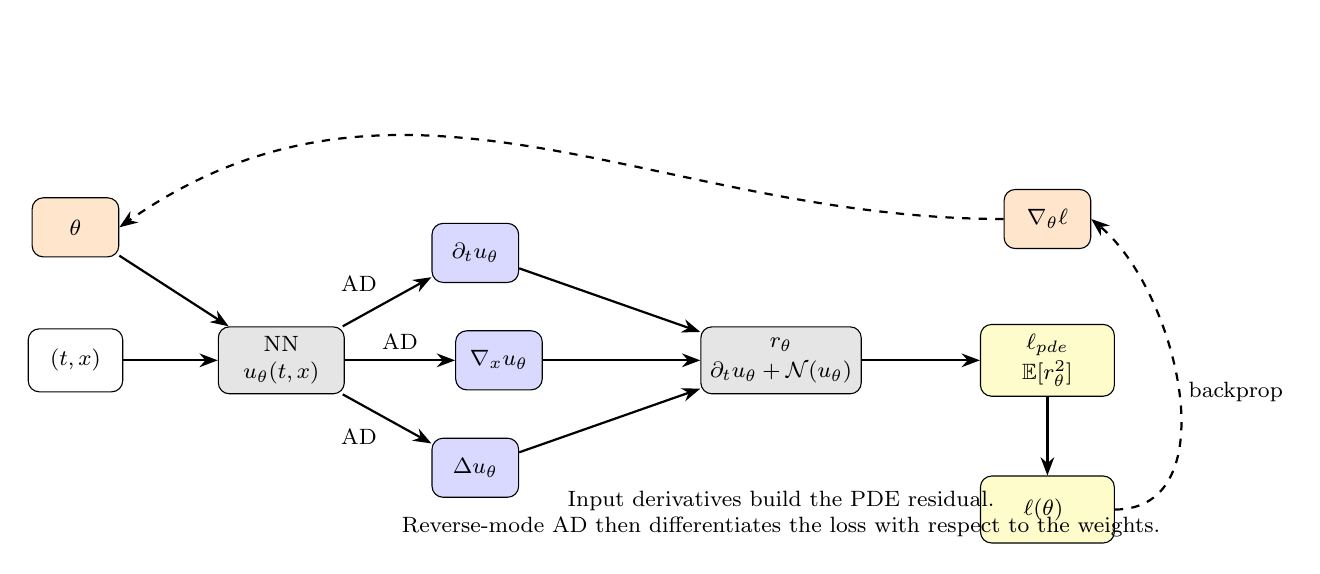
\begin{tikzpicture}[
  block/.style={rectangle, draw, rounded corners, minimum width=1.6cm, minimum height=0.85cm, align=center, fill=gray!20},
  input/.style={rectangle, draw, rounded corners, minimum width=1.2cm, minimum height=0.8cm, align=center, fill=white!20},
  param/.style={rectangle, draw, rounded corners, minimum width=1.1cm, minimum height=0.75cm, align=center, fill=orange!20},
  deriv/.style={rectangle, draw, rounded corners, minimum width=1.1cm, minimum height=0.75cm, align=center, fill=blue!15},
  loss/.style={rectangle, draw, rounded corners, minimum width=1.7cm, minimum height=0.85cm, align=center, fill=yellow!20},
  every node/.style={font=\footnotesize},
  arrow/.style={-Stealth, thick},
  rev/.style={-Stealth, thick, dashed}
]

% ------------------------------------------------------------
% Network evaluation
% ------------------------------------------------------------

\node[input] (xt) {$(t,x)$};
\node[param, above=0.9cm of xt] (theta) {$\theta$};

\node[block, right=1.2cm of xt] (nn) {NN\\$u_\theta(t,x)$};

\draw[arrow] (xt) -- (nn);
\draw[arrow] (theta) -- (nn);

% ------------------------------------------------------------
% Input derivatives
% ------------------------------------------------------------

\node[deriv, above right=0.55cm and 1.1cm of nn] (ut) {$\partial_t u_\theta$};
\node[deriv, right=1.4cm of nn] (ux) {$\nabla_x u_\theta$};
\node[deriv, below right=0.55cm and 1.1cm of nn] (uxx) {$\Delta u_\theta$};

\draw[arrow] (nn) -- node[above left] {AD} (ut);
\draw[arrow] (nn) -- node[above] {AD} (ux);
\draw[arrow] (nn) -- node[below left] {AD} (uxx);

% ------------------------------------------------------------
% PDE residual
% ------------------------------------------------------------

\node[block, right=2.0cm of ux] (res) {
$r_\theta$\\[0.05cm]
$\partial_t u_\theta+\mathcal N(u_\theta)$
};

\draw[arrow] (ut) -- (res);
\draw[arrow] (ux) -- (res);
\draw[arrow] (uxx) -- (res);

% ------------------------------------------------------------
% Loss
% ------------------------------------------------------------

\node[loss, right=1.5cm of res] (lpde) {
$\ell_{pde}$\\[0.05cm]
$\mathbb E[r_\theta^2]$
};

\node[loss, below=1.0cm of lpde] (lossbox) {
$\ell(\theta)$
};

\draw[arrow] (res) -- (lpde);
\draw[arrow] (lpde) -- (lossbox);

% ------------------------------------------------------------
% Backpropagation to parameters
% ------------------------------------------------------------

\node[param, above=0.95cm of lpde] (grad) {$\nabla_\theta \ell$};

\draw[rev] (lossbox.east) to[out=0,in=-40] node[right] {backprop} (grad.east);
\draw[rev] (grad.west) to[out=180,in=35] (theta.east);

% ------------------------------------------------------------
% Notes
% ------------------------------------------------------------

\node[align=center, below=1.1cm of res] {
Input derivatives build the PDE residual.\\
Reverse-mode AD then differentiates the loss with respect to the weights.
};

\end{tikzpicture}

\end{document}
